\chapter{Introduction}
\label{chpt:introduction}

Somatic cell division generates two genetically identical daughter cells from a single parent cell. Among different stages of the cell cycle, my thesis focus on mitosis. Mitosis follows the conclusion of interphase (during which nuclear DNAs are duplicated) and can be further divided into prophase, prometaphase (after the nuclear envelop breakdown and before all chromosomes are aligned at the metaphase plate, which is the main stage which my thesis revolves around), metaphase, anaphase, and telophase \cite{MBC4}.

To generate two genetically identical daughter cells, duplicated nuclear DNAs packed within chromosomes need to be distributed into the two daughter cells equally. This requires that each duplicated chromosome is stably attached to spindle microtubules emanating from the two opposite poles of the parent cell before the parent cell divides. The spindle assembly checkpoint (SAC) serves as a surveillance mechanism that monitors the completion of this process and prevents the premature onset of the anaphase, thereby avoiding chromosome missegregation \cite{MBC4}.

The SAC can robustly delay the onset of the anaphase in the presence of a single chromosome with monopolar attachment \cite{PtK1SingleUnattachedKT}. The question I want to address through my thesis research is how the SAC achieves such sensitivity. Through my extensive studies, I discovered that the SAC exploits cooperativity at multiple layers of the signaling cascade to achieve such sensitivity. This chapter introduces some of the basic facts, important concepts, and motivations of my thesis research to prepare my dear readers for later chapters. In later chapters, necessary information related to the experiments, reasoning, and discussion will be mentioned again or cross-referenced to the corresponding sections here.
% This is not intended to be a thorough literature review of every detail of the SAC.

\section{Spindle, kinetochore, and kinetochore-microtubule attachment}

To prepare for the equal distribution of duplicated nuclear DNAs packed within chromosomes, a mitotic cell forms the spindle (the green structure in \myref{SACRole}) whose microtubules attach to chromosomes from opposite poles of the cell. The adaptor structures on chromosomes which mediate such attachment are named kinetochores. After all chromosomes are bipolarly attached to the spindle and aligned at the metaphase plate (through a process named ``chromosome congression'' \cite{ChromosomeCongression}), the cell will enter the anaphase when sister chromatids separate from each other. The spindle will then pull the two sets of chromosomes towards opposite poles of the cell, which later become parts of the two daughter cells \cite{MBC4}.

\begin{figure}
    \centering
    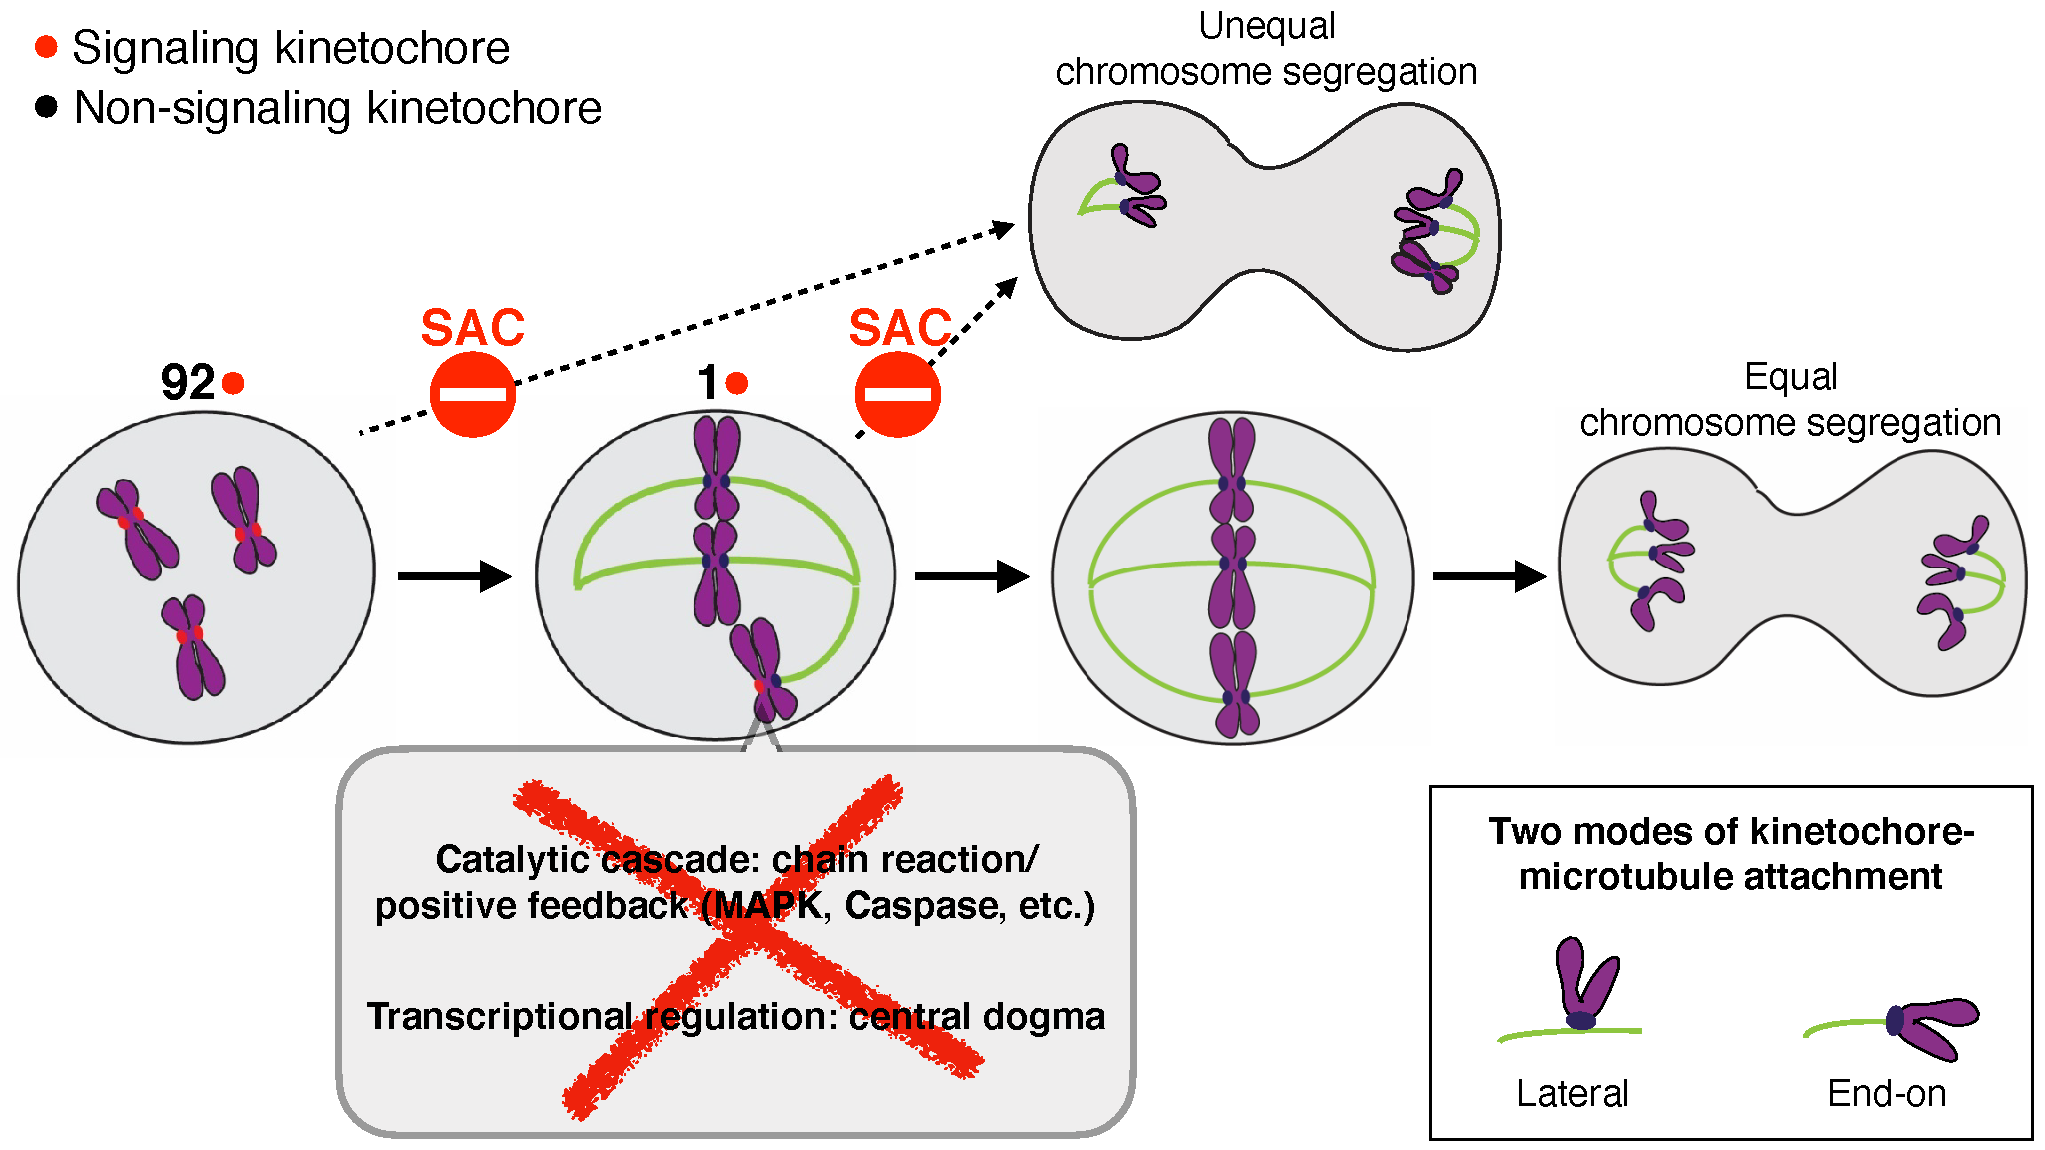
\includegraphics[width=\textwidth]{chapters/figures/SACRole.pdf}
    \caption{The gradual establishment of kinetochore-spindle microtubule attachment and the role of the spindle assembly checkpoint (SAC) in ensuring equal chromosome segregation.}
    \noindent\justifying In a canonical human somatic cell during mitosis, 46 chromosomes (with a total number of 92 chromatids and 92 kinetochores) gradually attach to the spindle during the prometaphase. Right after the nuclear envelop breakdown (NEBD) at the beginning of the prometaphase, all 92 kinetochores are not attached to microtubules. This number gradually decreases over the course of chromosome congression. Kinetochores without end-on microtubule attachment activate the SAC to prevent premature anaphase onset, ensuring equal distribution of chromosomes into daughter cells. Diagrams of the two modes of kinetochore-microtubule attachment (lateral vs end-on) are shown on the top right. It should be noted that lateral attachment is usually observed in the early stage of the establishment of kinetochore-microtubule attachment in the prometaphase, before sister chromatids separate from each other at the onset of the anaphase normally. The cartoon shows only one chromatid with one kinetochore in each case to simply demonstrate the concept.
    \label{SACRole}
\end{figure}

In most vertebrates, kinetochores range between 0.1--\SI{0.5}{\micro m} in diameter \cite{Rieder+Salmon1998}. The architecture of human kinetochores is proposed to resemble a Velcro-like interface, forming adaptable attachment sites for an average number of about 17 microtubules in the metaphase \cite{Wendell1993, Zaytsev2014, Zaytsev2015, Velcro, Kukreja2020}. There are two different modes of kinetochore-microtubule attachment in human cells: lateral attachment and end-on attachment (see \myref{SACRole}). The establishment of the kinetochore-microtubule attachment is a gradual and stochastic process \cite{GradualStochastic}.

% https://www.sciencedirect.com/science/article/pii/S0962892411000043: ...the interaction between kinetochores and spindle microtubules is stochastic [85–88], and sister kinetochores rarely attach to microtubules simultaneously.
% 85. Kirschner M., Mitchison T. Beyond self-assembly: from microtubules to morphogenesis. Cell. 1986;45:329–342.
% 86. Mitchison T., Kirschner M. Dynamic instability of microtubule growth. Nature. 1984;312:237–242.
% 87. Hayden J.H. Kinetochores capture astral microtubules during chromosome attachment to the mitotic spindle: direct visualization in live newt lung cells. J. Cell Biol. 1990;111:1039–1045.
% 88. Rieder C.L., Alexander S.P. Kinetochores are transported poleward along a single astral microtubule during chromosome attachment to the spindle in newt lung cells. J. Cell Biol. 1990;110:81–95.

Around a kinetochore in human cells, a crescent-shaped fibrous meshwork named the corona is assembled \cite{CoronaReview_Kops+Gassman2020}. It is formed through the polymerization of the ROD-Zwilch-ZW10-Spindly (RZZS) complex \cite{RZZS_Sacristan2018, RZZS_Raisch2022} and is stripped off the kinetochore by dynein at the establishment of microtubule attachment \cite{DyneinStripsCorona}. The corona expands the microtubule-attachment interface of a kinetochore and thereby facilitates the initial microtubule capture. The corona recruits the centromere-associated kinesin \protein{Cenp-E}, which promotes the conversion of lateral attachment into the desired end-on attachment \cite{Corona-CENP-E_Yao1997, GSK923295MonastrolCotreatment, CENPEActivity-BUBR1}. The corona also recruits \protein{Cenp-F} which may contribute to the stability of the kinetochore-microtubule attachment and limits the dynein-mediated stripping of the corona \cite{CENP-FLimitsStripping}.

\section{The spindle assembly checkpoint (SAC) signaling pathway in human cells}
%: the core pathway and the corona pathway
\label{TwoSACPathwaysIntro}

Cells deploy the spindle assembly checkpoint (SAC) to monitor the progress of the establishment of the kinetochore-microtubule attachment during the prometaphase. The SAC is activated at kinetochores without end-on microtubule attachment to block premature anaphase onset \cite{GSK923295MonastrolCotreatment, GSK923295LateralAttachmentEM, LateralAttachmentSAC}. This block allows time for the establishment of the end-on kinetochore-microtubule attachment. Once all attachment is secured, the SAC is silenced and the block is lifted \cite{SACActivationAndSilencing}. Mitosis is then resumed, heading toward equal segregation of chromosomes into daughter cells (see \myref{SACRole}).

After the NEBD, the SAC in mammalian cells relies on the kinetochore-localized signaling scaffold \protein{Knl1} as well as the corona during the prometaphase \cite{GSK923295LateralAttachmentEM, LateralAttachmentSAC, CoronaActivatesSAC}. We refer to them as the core pathway (which will be the main focus of my thesis; see \myref{CoreSAC}) and the corona pathway, respectively \cite{RZZ-MAD1vsBUB1-MAD1_2015, eSAC}.

\begin{figure}
    \centering
    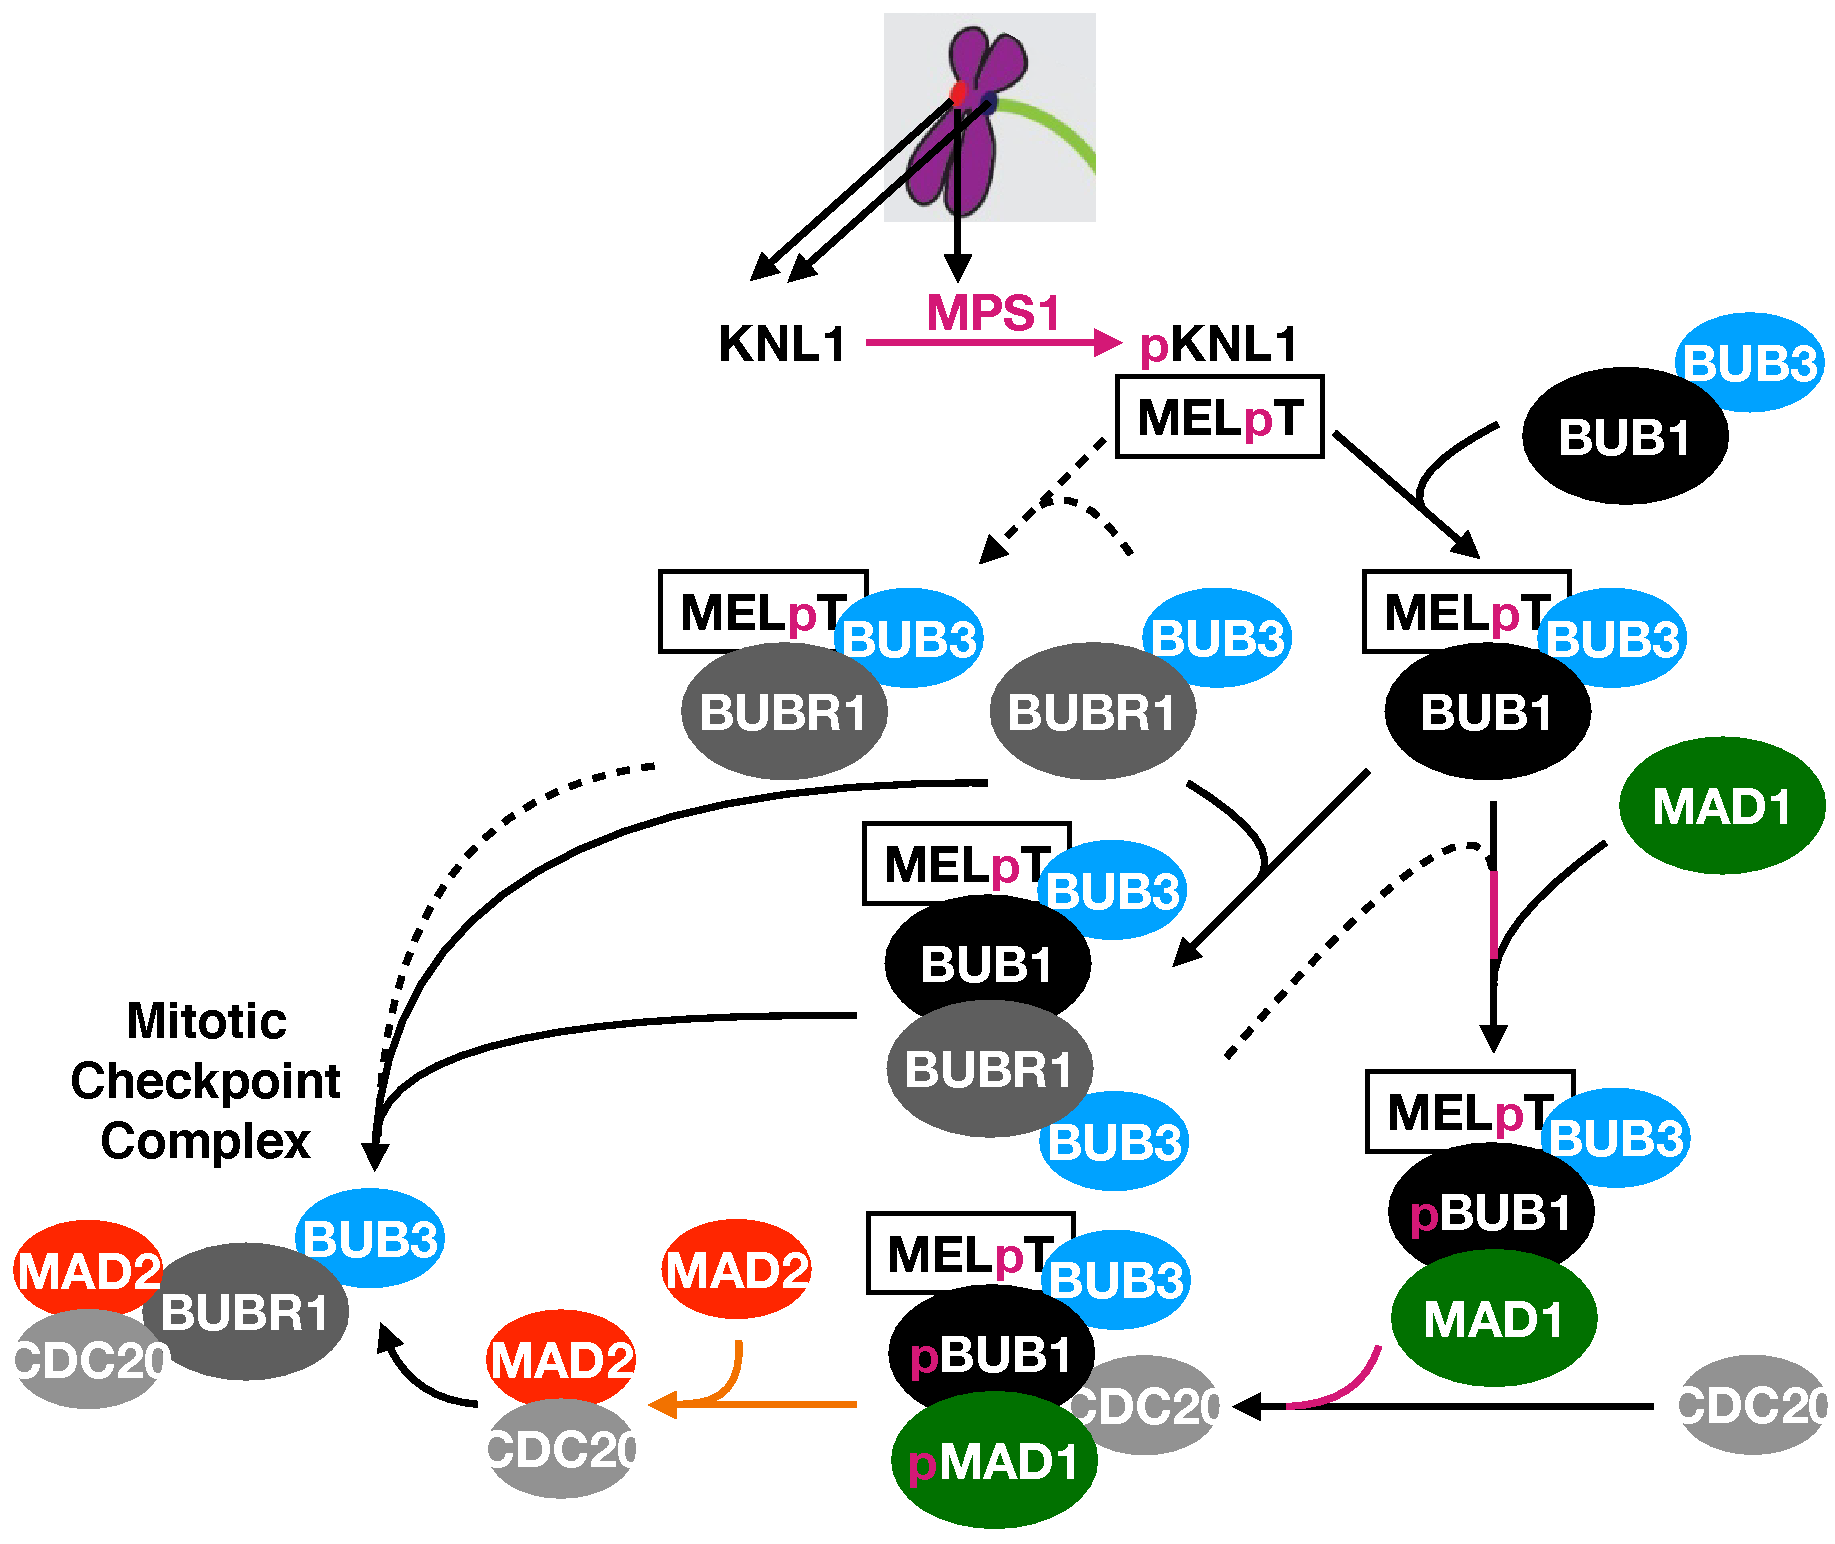
\includegraphics[width=0.94\textwidth]{chapters/figures/CoreSAC.pdf}
    \caption{The biochemical interactions and reactions of the core SAC signaling pathway.}
    \noindent\justifying In the core SAC signaling pathway, signaling kinetochores recruit the kinase \protein{Mps1} which phosphorylates the consensus MELT motifs on the scaffold protein \protein{Knl1}. Phosphorylated MELT motifs (the ``MELpT'' rectangle in the figure) will then recruit a series of SAC proteins and eventually generate the effector molecule known as the Mitotic Checkpoint Complex (MCC), which blocks the progression of mitosis. \protein{Cdc20} binds to signaling kinetochores cooperatively via its interactions with \protein{Bub1} and \protein{Mad1} \cite{BUB1-CDC20-MAD1, Tripartite}. Black solid arrows indicate direct binding or participation, which is either the consensus understanding in the field \cite{MPS1Localization_Ji, MPS1Localization_Hiruma, RecombinantKNL1, MELTActivity, BubBiochem, BubR1TwoPools, BUB1CD1-MAD1CStructure, Faesen2017, BUB1-CDC20-MAD1, Tripartite} or experimentally proved in my thesis research (see \myref{per_se}). Black dashed arrows indicate arguable \cite{BubBiochem, BubR1TwoPools} or hypothetical direct binding or participation. Magenta arrows and texts indicate \protein{Mps1} or involvement of \protein{Mps1}-mediated phosphorylation \cite{Ji2017eLife}. The orange arrow indicates catalytic reactions leading to the formation of the \protein{Cdc20}-\protein{Mad2} dimer, which will be the focus of \myref{chpt:4}. The green \protein{Mad1} oval indicates the \protein{Mad1}-\protein{Mad2} heterotetramer (see \myref{chpt:4}). This heterotetramer is extremely stable in the budding yeast \cite{StableHeterotetramer}. The molecular weight of \protein{Mad1} (an extended protein mainly composed of \textalpha{}-helices according to the prediction of AlphaFold \cite{AlphaFold}) is also much greater than the molecular weight of \protein{Mad2} (a globular protein \cite{Structure1GO4}). Therefore, the \protein{Mad1}-\protein{Mad2} heterotetramer is also sometimes simply referred to as ``\protein{Mad1}'' in the following context.
    \label{CoreSAC}
\end{figure}

The core SAC signaling pathway is scaffolded by \protein{Knl1} localized at all kinetochores. The human \protein{Knl1} possesses 19 consensus MELT motifs in its mostly discordered N-terminus and middle region \cite{MELTEvolution}, some of which are phosphorylated by the kinase \protein{Mps1} localized at signaling kinetochores \cite{MPS1-KNL1_London2012, MPS1-KNL1_Shepperd2012, MPS1-KNL1_Yamagishi2012, MPS1Localization_Ji, MPS1Localization_Hiruma}. These phosphorylated MELT motifs initiate the core SAC signaling pathway by recruiting SAC proteins like \protein{Bub3}, \protein{Bub1}, \protein{BubR1}, \protein{Cdc20}, and the \protein{Mad1}-\protein{Mad2} heterotetramer, thereby promoting the assembly of the mitotic checkpoint complex (MCC) consisting of \protein{BubR1}/\protein{BubR1}-\protein{Bub3} and \protein{Cdc20}-\protein{Mad2} \cite{RecombinantKNL1, MELTActivity, BubBiochem, BubR1TwoPools, BUB1CD1-MAD1CStructure, Faesen2017, BUB1-CDC20-MAD1, Tripartite, SpMCC} (see \myref{mNG-BUBR1_NocWashoutMontage}). The mitotic checkpoint complex inhibits the E3 ubiquitin ligase anaphase-promoting complex/cyclosome (APC/C) \cite{APC-MCC_Alfieri2016, APC-MCC_Yamaguchi2016}. APC/C ubiquitinates Cyclin B1, a key mitosis regulator, thereby targeting it for proteasome-mediated degradation \cite{CyclinB1Degradation_Clute+Pines1999, CyclinB1Degradation_Chang2003, SeparaseStructure}. Through the inhibition of the APC/C, the degradation of Cyclin B1 is suppressed and the onset of anaphase is delayed.

In the corona pathway of the SAC, the corona recruits the \protein{Mad1}-\protein{Mad2} heterotetramer to signaling kinetochores and promotes the SAC signaling activity \cite{CoronaActivatesSAC}. It should be noted that the core pathway and the corona pathway are not independent in human cells. Corona constituents \protein{Cenp-E} and \protein{Cenp-F} interact with core SAC pathway components \protein{BubR1} and \protein{Bub1}, respectively \cite{CENPELocalization-BUBR1, CENP-FLimitsStripping}. It has also been suggested that the recruitment of \protein{Mad1} to signaling kinetochores may be cooperative, facilitated by both the corona and \protein{Bub1} \cite{MIS12-CEP57-MAD1-MAD2, siROD_Zhang2019}. We conceptually separate the two pathways because the corona does not exist in the budding yeast, while the core pathway is conserved from yeast to human \cite{YeastNoRZZ}.

The MCC is also assembled at the nuclear pore complex (NPC) during the interphase and prophase, where the \protein{Mad1}-\protein{Mad2} heterotetramer is recruited by the nuclear basket protein \protein{Tpr} \cite{TPR-MAD1_Lee2008, PremitoticMCC}. Little is known about the regulations and mechanisms of the MCC assembly at the NPC, but it has been suggested to provide cells that newly enter the prometaphase with a starting pool of MCC and contribute to the robustness of the SAC.

\section{The sensitivity and responsiveness of the SAC}
\label{Sensitivity+Responsiveness}

The SAC signaling activity is positively correlated with the total number of signaling kinetochores \cite{RiederNormalProgression, Rheostat, Ablation}. However, even a single unattached kinetochore delays anaphase onset in a mammalian somatic cell line \cite{PtK1SingleUnattachedKT}. Although the biochemical interactions and reactions of the SAC signaling pathway have been mostly elucidated, how a single unattached kinetochore can delay anaphase onset has not been studied thoroughly. Understanding how the SAC achieves such sensitivity requires a quantitative and systematic examination of the SAC signaling pathway.

Signaling pathways may boost its sensitivity to a modest input by many mechanisms. Some signaling pathways amplify the input via biochemical reactions while some attain ultrasensitivity featuring a switch-like sigmoidal dose-response relationship (see \myref{CurveTypes}). Due to the probable lack of amplification mechanisms in the SAC signaling pathway (see the caption of \myref{SACNoAmplification} for detailed explanations), my focus is to study whether and how the SAC realizes ultrasensitivity (see \myref{Cooperativity-Ultrasensitivity} for details).

\begin{figure}
    \centering
    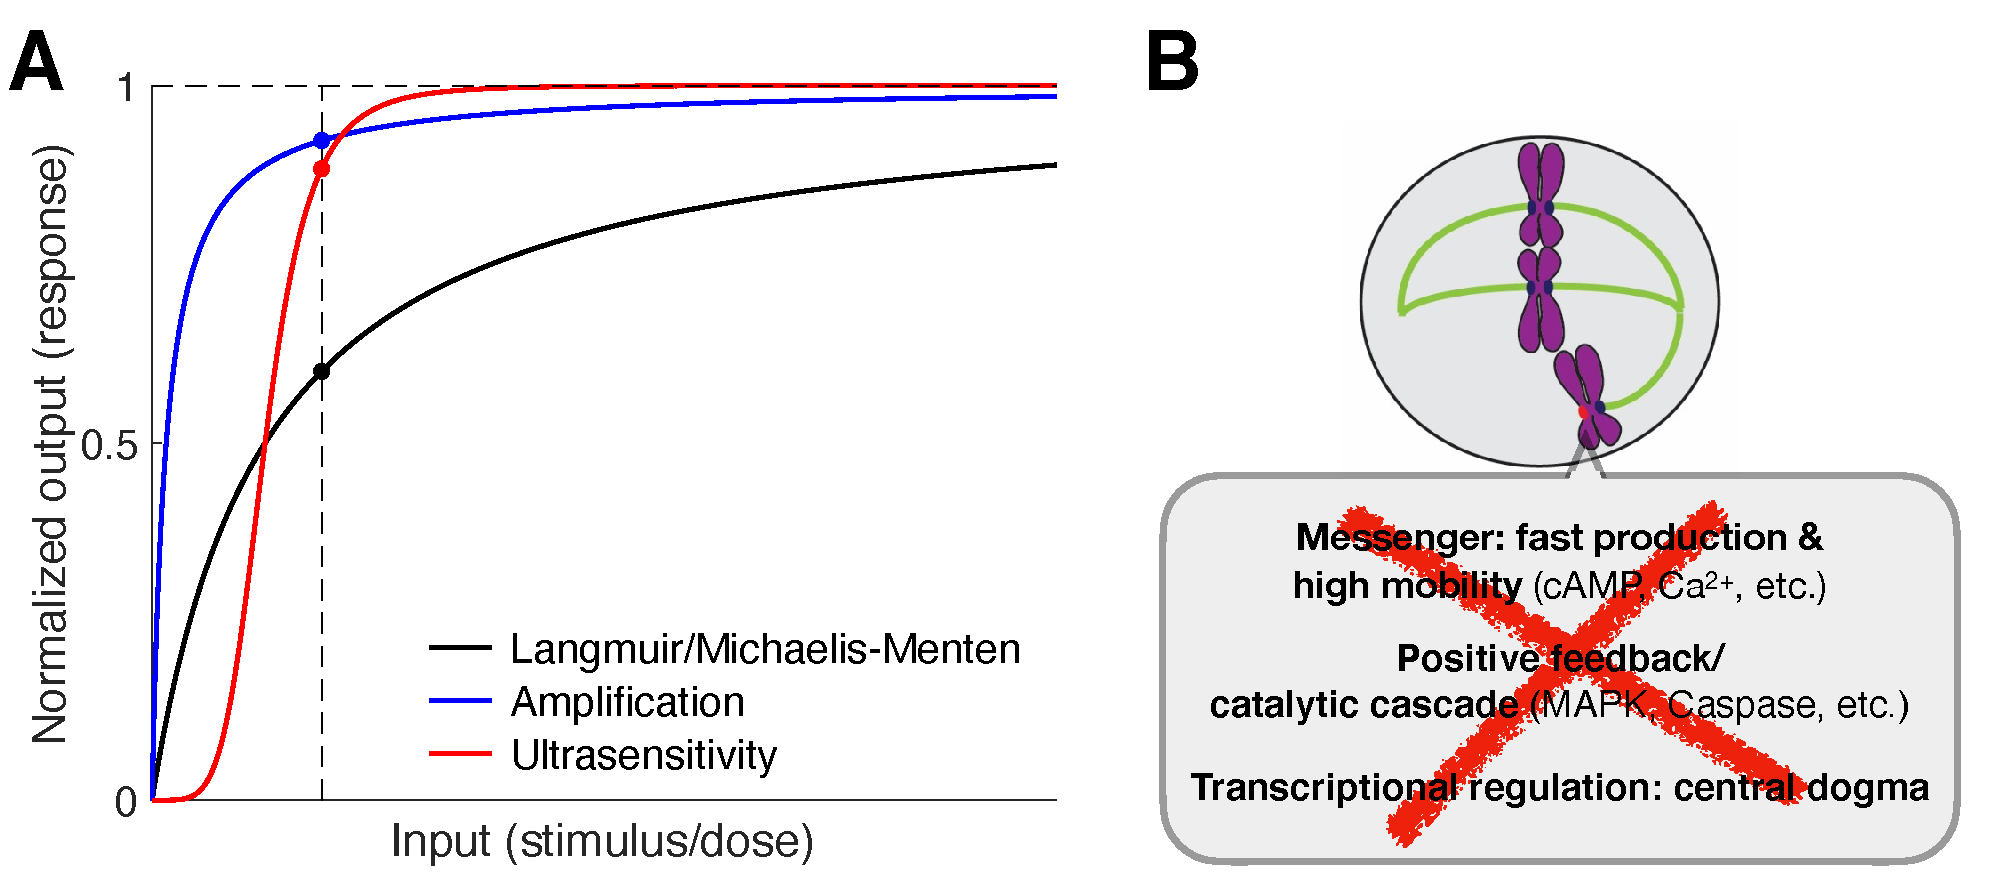
\includegraphics[width=\textwidth]{chapters/figures/SensitivityMechanisms.pdf}
    \phantomsubfiglabel{CurveTypes} % subfigure A
    \phantomsubfiglabel{SACNoAmplification} % subfigure B
    \caption{Many mechanisms may realize the sensitivity of a signaling pathway to a modest input.}
    \noindent\justifying 
    (A) A signaling pathway may boost its sensitivity to a modest input by signal amplification (via, for example, a second messenger, a catalytic cascade, positive feedback, or the central dogma; the blue curve) or ultrasensitivity (the red curve). The blue curve is derived by compressing the vanilla relationship of the Langmuir adsorption equation and Michaelis-Menten kinetics (the black curve) in the horizontal direction by the amplification factor. (B) Many well-characterized signal amplification mechanisms do not apply to the SAC. The smallest molecule in the core SAC signaling pathway (other than the ATPs in the phosphorylation reactions; see \myref{CoreSAC}) is \protein{Mad2}, whose canonical isoform (\SI{23.5}{kDa}) is still much larger than typical second messengers. However, \protein{Mad2} in the cell may be catalyzed to undergo a conformational switch to interact with \protein{Cdc20} (and form the MCC subcomplex \protein{Cdc20}-\protein{Mad2}) as well as many proteins, thereby regulating mitosis from various aspects \cite{Separase-SGO2-MAD2, KIF20A-MAD2, CyclinB2-MAD2}. This catalysis may constitute a signal amplification mechanism that contributes to the sensitivity of the SAC (see \myref{chpt:4}). No catalytic cascade has been identified that could amplify the SAC signaling activity. Also, there has been no report on positive feedback in the core SAC signaling pathway (while several cases of negative feedback regulations have been indicated \cite{Mps1pAutophosphorylation, PP2ADephosphorylatesBUB1, PP2ADephosphorylatesKNL1, PP2A-B56}). Finally, transcriptional regulations that amplify inputs through the central dogma (or realize ultrasensitivity through the potential oligomerization or allosteric regulations of the transcriptional factors \cite{TFMultimerization, TFAllostericRegulation}) are also unlikely because the genome is highly condensed during the prometaphase.
    \label{SensitivityMechanisms}
\end{figure}

After all chromosomes are attached to spindle microtubules, the SAC is deactivated and SAC proteins are stripped or released from signaling kinetochores (see \myref{mNG-BUBR1_NocWashoutMontage}). The block inflicted on the progression of mitosis is lifted \cite{PP2A-B56, DyneinStripsCorona, BubR1MitosisTurnover, CCT-MCCDisassembly, Ubiquitylation-MCCDisassembly, UBR5-MCCDisassembly, TRIP13-p31-MAD2, APC-SUMO}. A previous study has found that sister chromatids separate from each other in about half an hour after all chromosomes are attached to spindle microtubules in a mammalian cell line \cite{RiederNormalProgression}, demonstrating the responsiveness of the SAC. It is important to note (for the discussions in later chapters) that during normal mitosis, the prometaphase arrest is released without all kinetochores fulfilling their maximum microtubule-binding capacity. There is also a small amount of certain SAC proteins remaining at metaphase and anaphase kinetochores \cite{SACSilencing_Etemad2019, SACSilencing_Kuhn2019}.

\begin{figure}
    \centering
    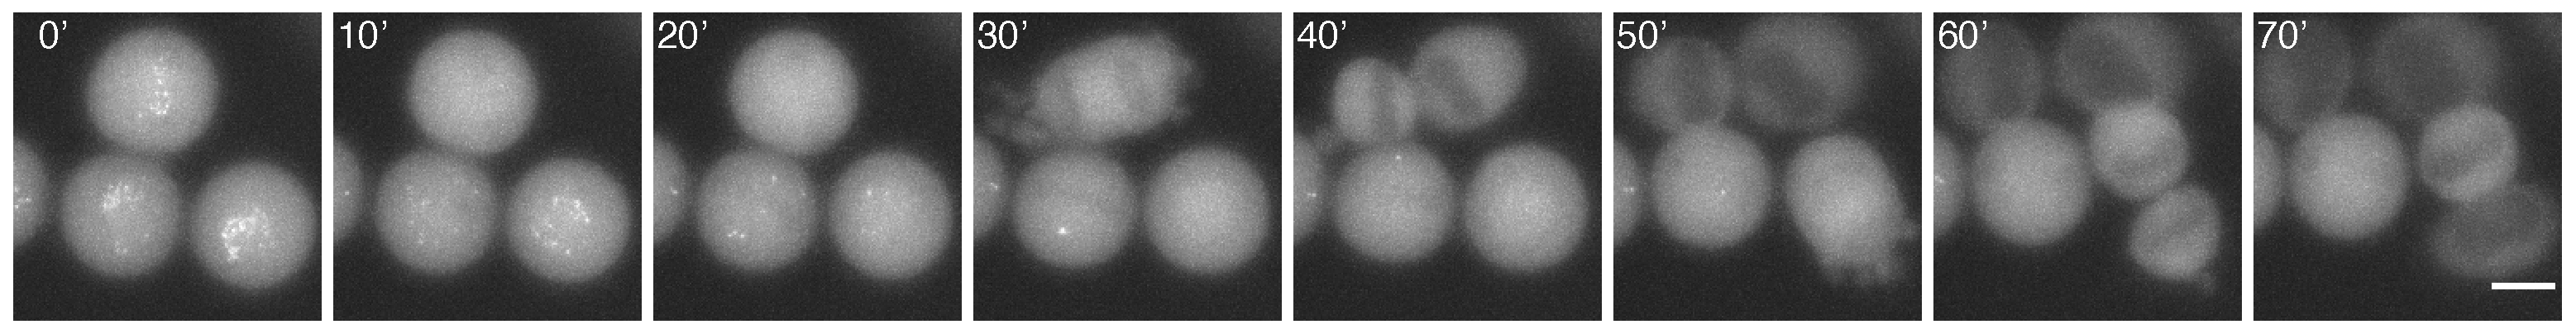
\includegraphics[width=\textwidth]{chapters/figures/mNG-BUBR1_NocWashoutMontage.pdf}
    \caption{Recruitment of \protein{BubR1}, a SAC protein, at nocodazole-induced signaling kinetochores and the release of \protein{BubR1} from kinetochores at the deactivation of the SAC before the anaphase onset.}
    \noindent\justifying Live genome-edited mNG-\gene{BubR1} cells (see \myref{TaggingSACProteins,CRISPRMethods}) were first arrested in mitosis by nocodazole (see \myref{TechnicalChallenges}), then released into drug-free FluoroBrite\texttrademark{} DMEM [Gibco; supplemented with 9\% (by volume) of fetal bovine serum and $1\times$ GlutaMAX] before the start of imaging (labeled as `` 0' ''), and finally imaged on a wide-field Nikon Eclipse Ti-E/B inverted microscope equipped with a Nikon Plan Fluor $40\times$, 0.75 NA objective (see \myref{chpt3ImagingMethods}). The intermediate magnification selector knob was switched to $1.5\times$. Cells that were released from the nocodazole arrest resumed the progression of mitosis \cite{Kukreja2020}. A montage of the maximum $z$-projection taken from the same field of view in the green fluorescence channel is shown here. The bright spots in the cell indicate the recruitment of mNG-\protein{BubR1} onto signaling kinetochores. These spots disappeared over time before the anaphase onset because the SAC was silenced once the kinetochore established end-on attachment to spindle microtubules. Scale bar, \SI{10}{\micro m}.
    \label{mNG-BUBR1_NocWashoutMontage}
\end{figure}

Although the responsiveness of the SAC is not the focus of my thesis, the sensitivity and responsiveness of the SAC are like two sides of the same coin \cite{eSAC}. Understanding the origin of the sensitivity and responsiveness of the SAC and their balancing (see \myref{eSACDiscussions}) will help us better comprehend how the SAC activates to prevent premature anaphase onset in the presence of a decreasing number of signaling kinetochores and silences to initiate anaphase onset after all chromosomes are attached to spindle microtubules promptly during normal mitosis.

\section{Cooperativity is one way to realize ultrasensitivity}
\label{Cooperativity-Ultrasensitivity}

The widely applicable Langmuir adsorption equation and Michaelis-Menten kinetics in biochemical interactions or reactions commonly inflict a dampening effect on any changes in the input \cite{CooperativityQA}. To explain such dampening effect, suppose that the output $f(x) \geq 0$ is a monotonically increasing and strictly concave function of the input $x$ for all $x \geq 0$ (like the Langmuir adsorption equation and Michaelis-Menten kinetics) and that the output is 0 if and only if the input is 0. Comparing the outputs [$f(x_2)$ and $f(x_1)$] corresponding to the inputs ($x_2 > x_1 > 0$), we have

\begin{equation*}
    1 < \dfrac{f(x_2)}{f(x_1)} = \dfrac{f(x_2)}{f[\dfrac{x_1}{x_2} \cdot x_2 + (1-\dfrac{x_1}{x_2}) \cdot 0]} < \dfrac{f(x_2)}{\dfrac{x_1}{x_2}f(x_2) + (1-\dfrac{x_1}{x_2})f(0)} = \dfrac{x_2}{x_1},
\end{equation*}

\noindent which states that the contrast between the outputs is less than the contrast between the inputs \cite{InhibitorUltrasensitivity}.

There are many well-studied mechanisms deployed by signaling cascades to circumvent the dampening effect and sensitize the output \cite{ZeroOrder, MultistepUltrasensitivity, Bistability}. For example, the multi-step/multi-site phosphorylation mechanism has been implied in the SAC by experimental evidence \cite{Ji2017eLife} (see the magenta arrows and texts in \myref{CoreSAC}). Such mechanism enables a sigmoidal dose-response relationship, which is named ``ultrasensitivity'' (red curve). The advantage of ultrasensitivity compared to simple signal amplification is that the signaling response is robust against a small noise (during the activation stage) or residue (during the deactivation stage) in the input (see \myref{CurveTypes}). Such robustness may be exploited by the SAC to realize its responsiveness mentioned above.

%Here in my thesis, I will focus on the implied role of cooperativity in the SAC.
Another way to realize ultrasensitivity is cooperativity. ``Cooperativity'' was originally used to describe the binding of oxygen molecules to the multi-subunit hemoglobin \cite{KNF, MWC}. Hereafter, I will use the term ``positive cooperativity'' (or simply ``cooperativity'') to describe the phenomenological synergy, which I attribute to the increased local concentration of SAC proteins due to their co-localization on the same signaling scaffold (see the descriptions of the proposed models in \myref{ProzoneEffectModel,FinalKnittingModel}). This is reminiscent of the theoretical explanation of the avidity between antibodies and antigens \cite{AvidityMath}, another well-characterized example of cooperativity.

\section{Studying the SAC quantitatively \Latin{in vivo}: complications, challenges, and methodology}
\label{TechnicalChallenges}

Studying the SAC quantitatively \Latin{in vivo} is hindered by many intrinsic complications and technical challenges. First, as introduced in \myref{TwoSACPathwaysIntro}, the SAC signaling cascade is physically confined at kinetochores. There, the potential molecular crowding may slow down diffusion due to increased local viscosity, thereby reducing reaction rates; on the other hand, the potential increase of the effective concentration of reactants may increase reaction rates \cite{MolecularCrowding}. \Latin{In vitro} reconstitution of the SAC signaling cascade using purified proteins may not faithfully reflect the biophysical aspects of the kinetochore environment.

Second, the biochemical cascade of the SAC is regulated by many other kinases as well as phosphatases in human cells. Some of them are recruited by kinetochore proteins that are not an integral part of the core SAC pathway, while others directly bind to SAC proteins. For example, both \protein{Plk1} and Aurora B are important kinases that regulate mitosis. \protein{Plk1} directly binds to \protein{Bub1} and the kinetochore protein \protein{Cenp-U} \cite{CENPU+BUB1-PLK1}, while Aurora B localizes predominantly to the inner centromere during the prometaphase \cite{BUB1_pH2A_AuroraB}. Another example is that \protein{BubR1} directly binds to PP2A-B56, a phosphatase that silences the SAC either directly \cite{PP2ADephosphorylatesKNL1, PP2ADephosphorylatesBUB1} or indirectly \cite{BUBR1_KT-MT, Suijkerbuijk2012, BUBR1-L669A+I672A, PP2A-B56-BUBR1ChromosomeCongression_Xu2013, PP2A-B56}. These interactions and regulations complicate the design of \Latin{in vivo} experiments and the interpretation of cell biology data (for example, see \myref{per_se}).

Third, as addressed in \myref{TwoSACPathwaysIntro}, the core pathway and the corona pathway of the SAC are not independent in human cells. Our understanding of the architecture of either the kinetochore or the corona is still far from complete. Dissecting the two pathways properly may be necessary to study the origin of the sensitivity of the SAC in human cells.

Fourth, to study the origin of the sensitivity of the SAC in human cells, we need to create the scenario wherein mitotic cells have a small number of signaling kinetochores. Very few studies have attempted it \cite{RiederNormalProgression, Rheostat, Ablation}. In some of these studies, the researchers either (1) treated cells with a low concentration of microtubule drugs and specifically looked for cells with a small number of signaling kinetochores, or (2) employed laser microsurgery to cut microtubules that attached to kinetochores. These strategies may not be robust or require specialized microscopy setups. More importantly, they do not provide enough data throughput to counter the stochastic nature of the establishment of the kinetochore-microtubule attachment \cite{GradualStochastic}.

Finally, over-expression of a SAC protein that is commonly observed in transgenic cells may deplete the cytosolic pool of the corresponding binding partner, thereby impairing the SAC signaling activity \cite{Bub3Competition, FissionYeastSACRobustness, ATMPhosphorylatesMad1S214, MAD1Overexpression_Ryan2012}. On the other hand, the SAC signaling activity maintains at a considerable level even when most \protein{Bub1} \cite{Raaijmakers2018, RZZ-MAD1vsBUB1-MAD1_2018, siROD_Zhang2019} or \protein{Mad1} (see \myref{chpt:4}) proteins are knocked down. These factors make it hard to execute a knockdown-rescue experiment.

We adopted or developed many experimental methods to circumvent the aforementioned complications and challenges. To dissect the role of the core SAC pathway without the complication of kinases recruited by kinetochore proteins or the corona pathway, we engineered an ectopic SAC (eSAC) activator consisting of a recombinant \protein{Knl1} phosphodomain and a recombinant \protein{Mps1} kinase domain (see \myref{chpt:2} for details). The eSAC activator hijacks the endogenous SAC signaling pathway and can be easily quantified. Combined with a semi-automatic data analysis pipeline which I developed, this novel tool offers the capability to process large live-cell imaging data sets to reveal the dose-response characteristics of the core SAC signaling pathway.

To visualize and quantify the localization of SAC proteins at signaling kinetochores without disrupting the expression patterns of these SAC proteins, we utilized CRISPR-Cas9-mediated genome editing to tag SAC genes \Latin{in situ} \cite{CRISPRProtocol}. This strategy may protect any endogenous transcriptional and translational regulations. The resulting genome-edited cell lines may also serve as a standard in filtering cells with induced expression of SAC proteins at various levels in a knockdown-rescue experiment (see \myref{chpt:3,chpt:4} for details).

To study the correlations between the amount of SAC proteins localized to each signaling kinetochore and the total number of signaling kinetochores, we treated the cells with either GSK923295 or nocodazole (see \myref{chpt:3} for details). GSK923295 inhibits the ATPase activity of \protein{Cenp-E}, thereby disrupting chromosome congression and yielding small numbers of chromosomes near spindle poles \cite{GSK923295}. These polar chromosomes typically possess one kinetochore that is unattached or laterally attached to spindle microtubules and activates the SAC \cite{GSK923295MonastrolCotreatment, GSK923295LateralAttachmentEM, LateralAttachmentSAC}. Nocodazole affects the dynamics of microtubules and distorts spindles in human cells \cite{TypeIIISpindle_330nMNoc, RZZ-MAD1vsBUB1-MAD1_2015}. At the most commonly used concentration of \SI{330}{nM}, nocodazole treatment turns on SAC signaling at almost all kinetochores. In general, the effect of nocodazole can range from creating a small number of unattached kinetochores at a low dosage (see \cite{Ablation, RZZ-MAD1vsBUB1-MAD1_2015} or \myref{per_se}) to completely nullifying the formation of any microtubules at a high dosage (like \SI{6.6}{\micro M} used in \myref{MPS1sen-KTSection}).